\section{Visualisation du corpus dans PixPlot}

\begin{figure}[H]
    \centering
    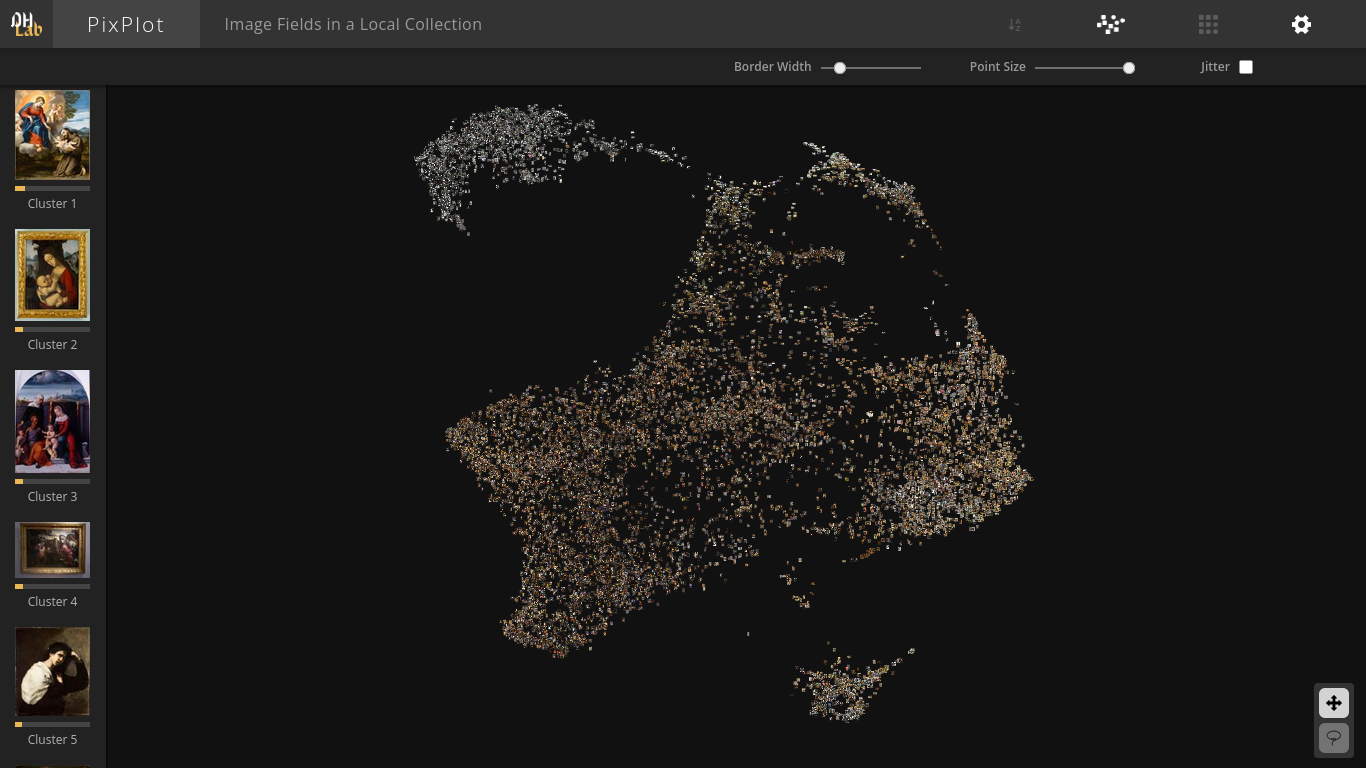
\includegraphics[width=1\textwidth]{annexes/figures/PP-generale.png}
    \caption{Visualisation générale des tableaux du RETIF dans PixPlot.}
    \label{fig:PP-general}
\end{figure}

\begin{figure}[H]
    \centering
    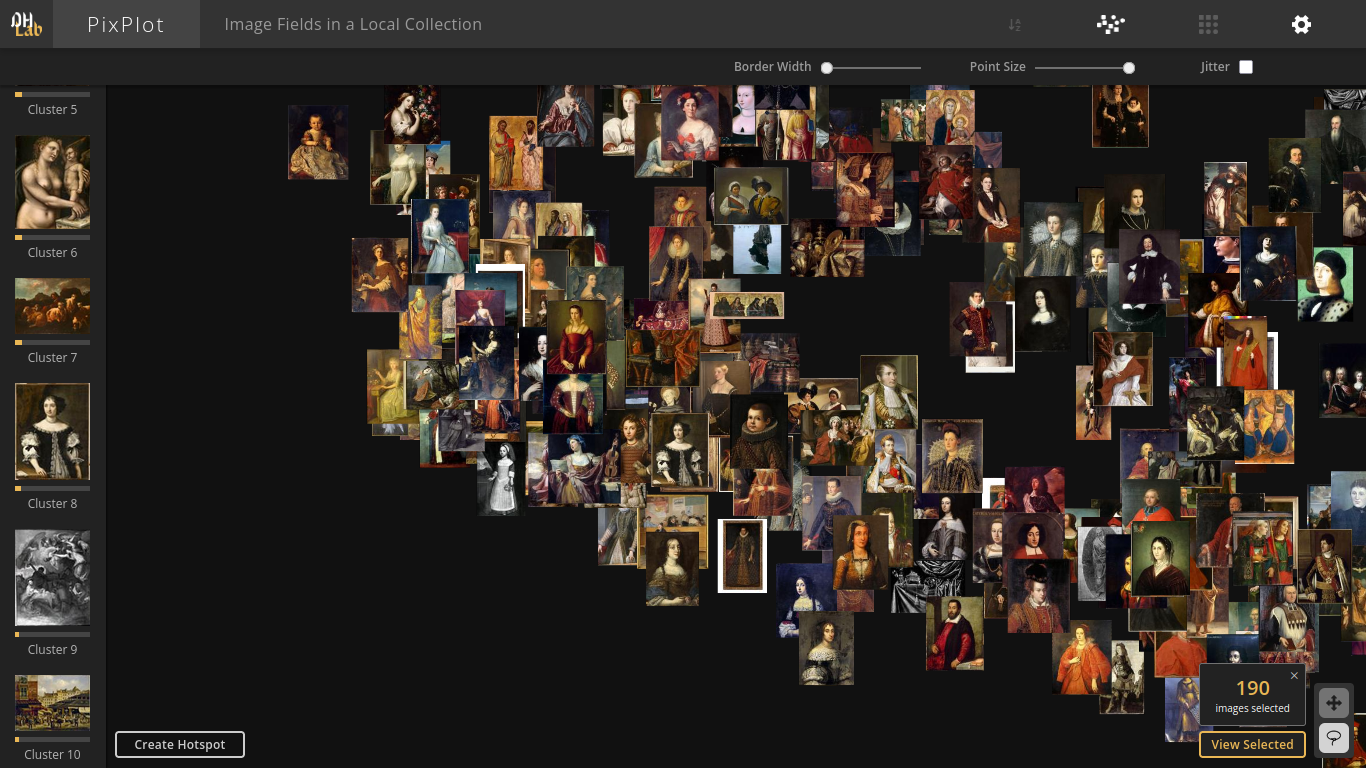
\includegraphics[width=1\textwidth]{annexes/figures/PP-portraits.png}
    \caption{Cluster de portraits identifié dans l'angle inférieur gauche de la visualisation du RETIF dans PixPlot.}
    \label{fig:PP-portraits}
\end{figure}

\begin{figure}[H]
    \centering
    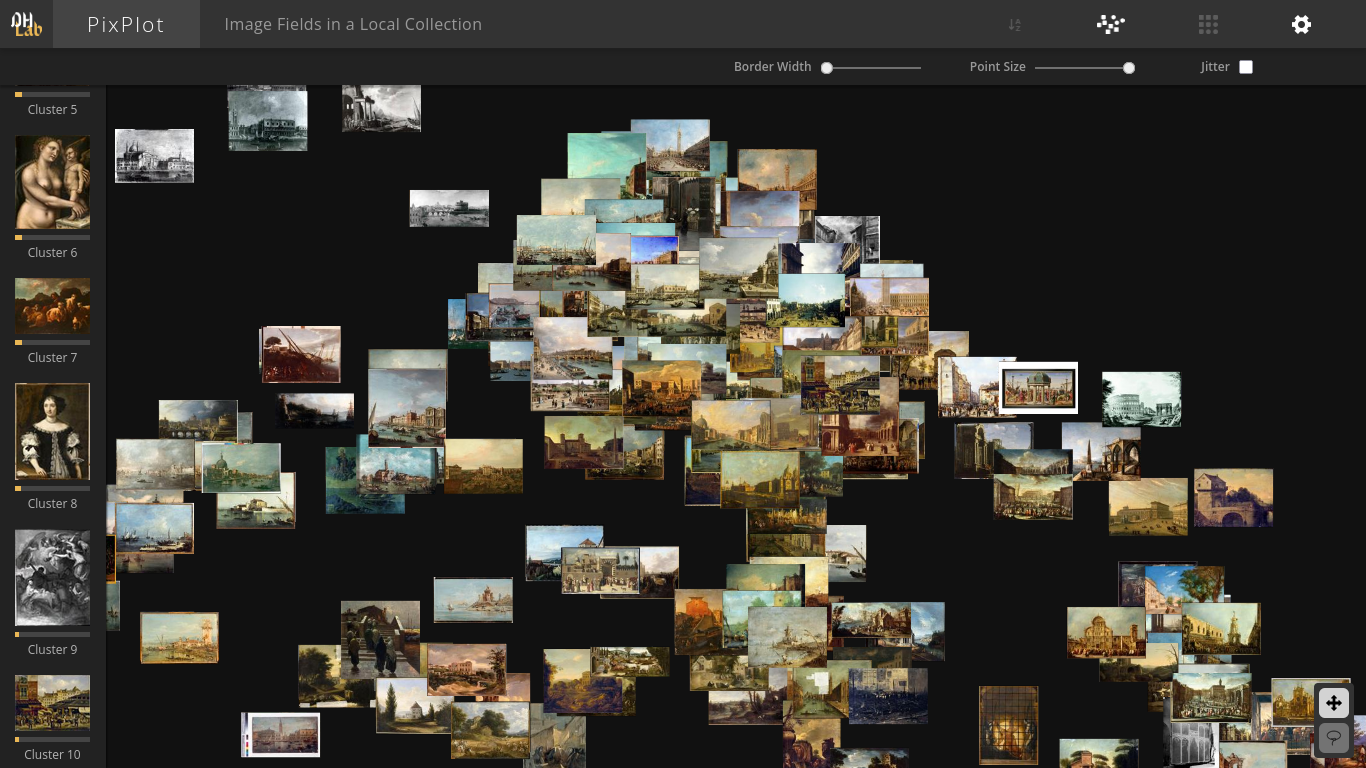
\includegraphics[width=1\textwidth]{annexes/figures/PP-vedute.png}
    \caption{Cluster de paysages urbains dans l'angle supérieur droit de la visualisation du RETIF dans PixPlot.}
    \label{fig:PP-vedute}
\end{figure}

\begin{figure}[H]
    \centering
    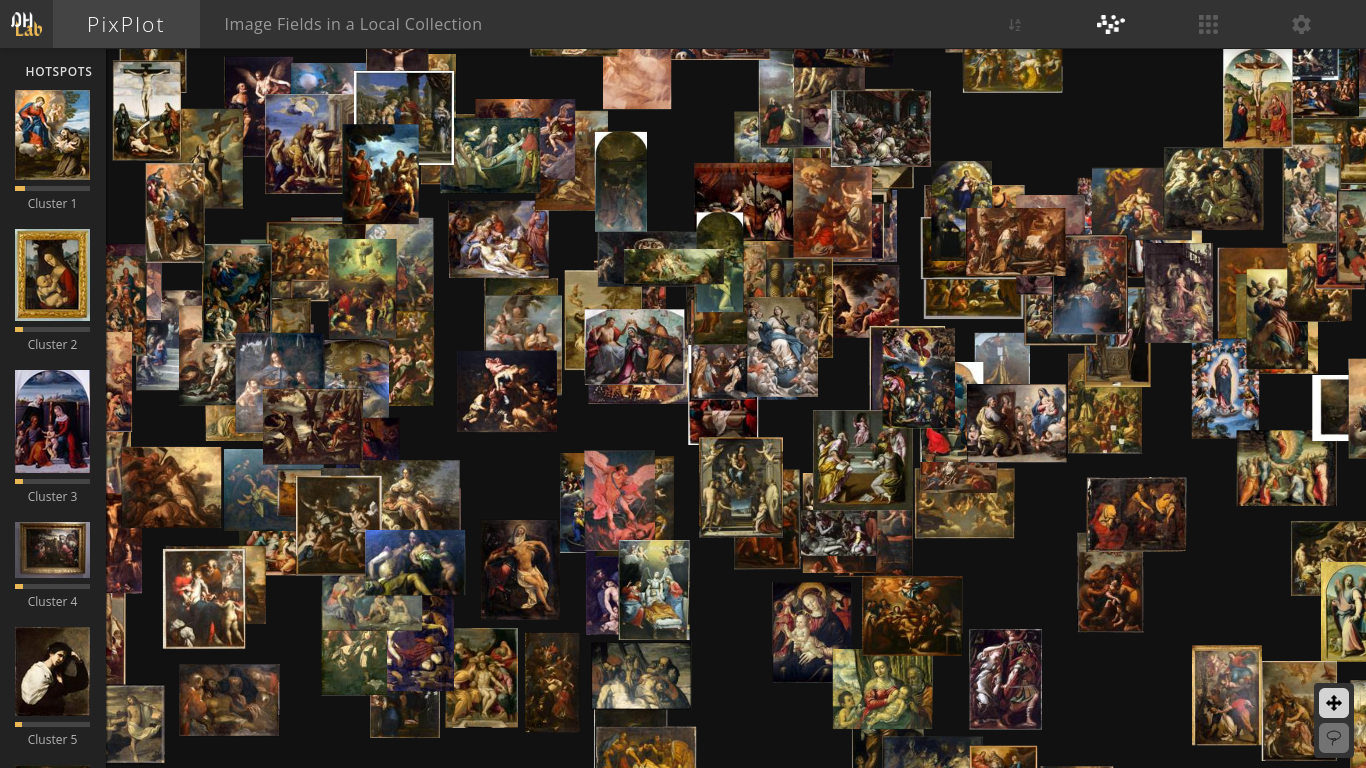
\includegraphics[width=1\textwidth]{annexes/figures/PP-scenes.png}
    \caption{Cluster des scènes religieuses et mythologiques au centre de la visualisation du RETIF dans PixPlot.}
    \label{fig:PP-scenes}
\end{figure}

\begin{figure}[H]
    \centering
    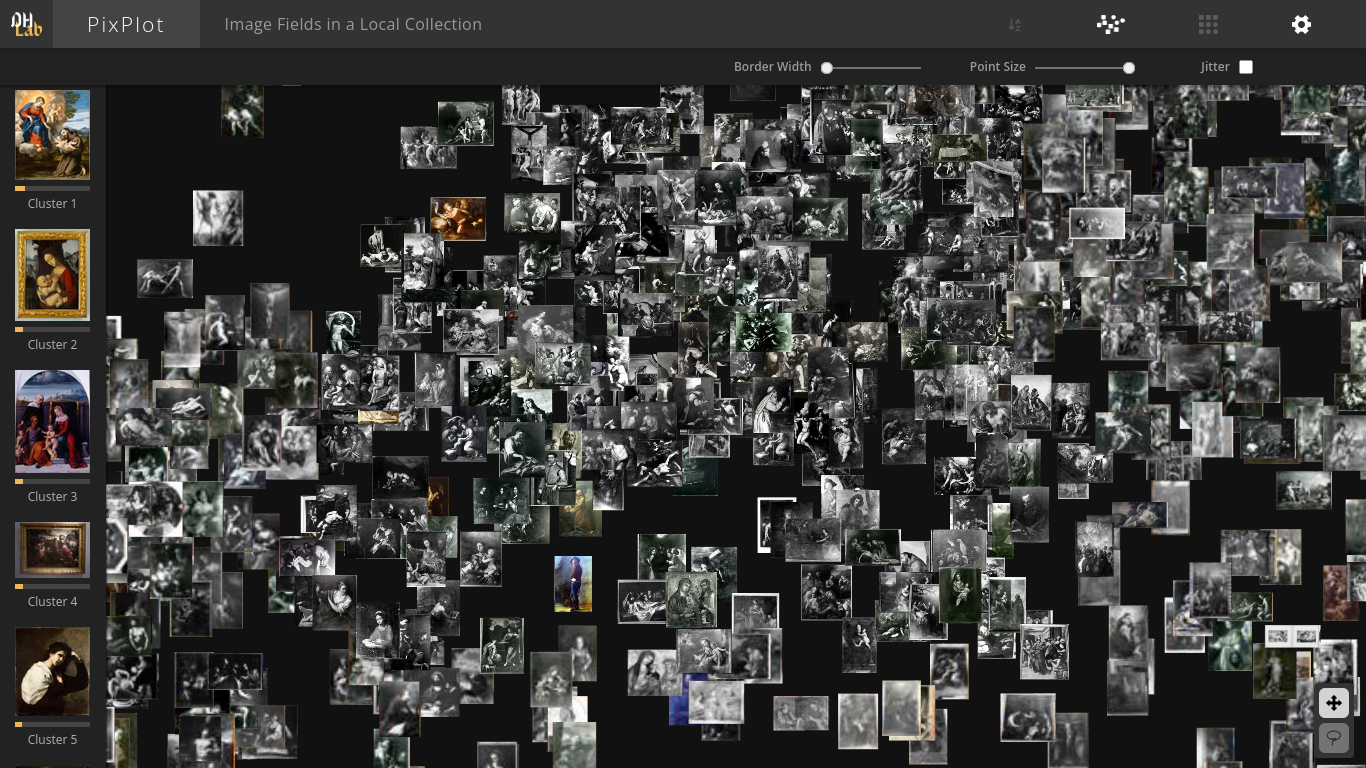
\includegraphics[width=1\textwidth]{annexes/figures/PP-n&b.png}
    \caption{Cluster des photographies en noir et blanc dans l'angle supérieur gauche de la visualisation du RETIF dans PixPlot.}
    \label{fig:PP-n&b}
\end{figure}

\begin{figure}[H]
    \centering
    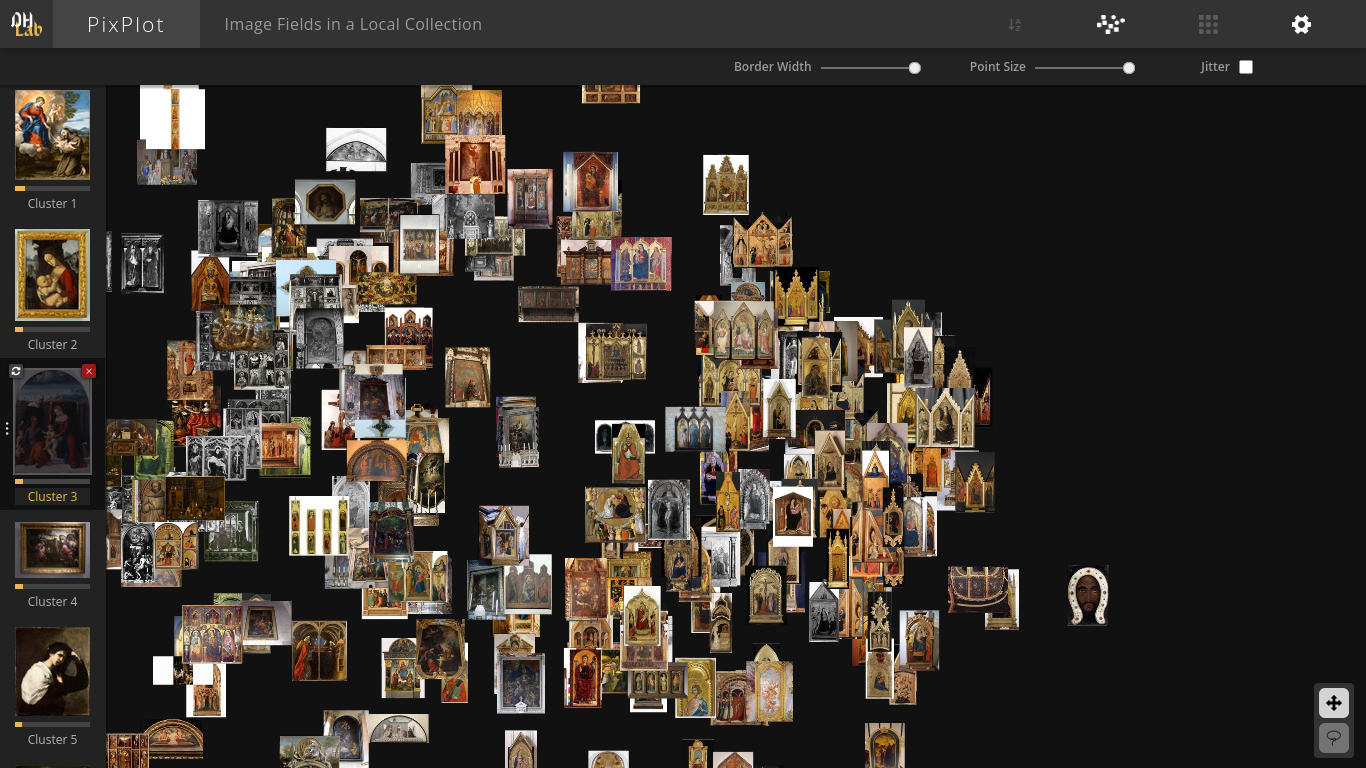
\includegraphics[width=1\textwidth]{annexes/figures/PP-polyptiques.png}
    \caption{Cluster des panneaux médiévaux et des tableaux dans leur contexte dans le bord droit  de la visualisation du RETIF dans PixPlot.}
    \label{fig:PP-polyptiques}
\end{figure}

\begin{figure}[H]
    \centering
    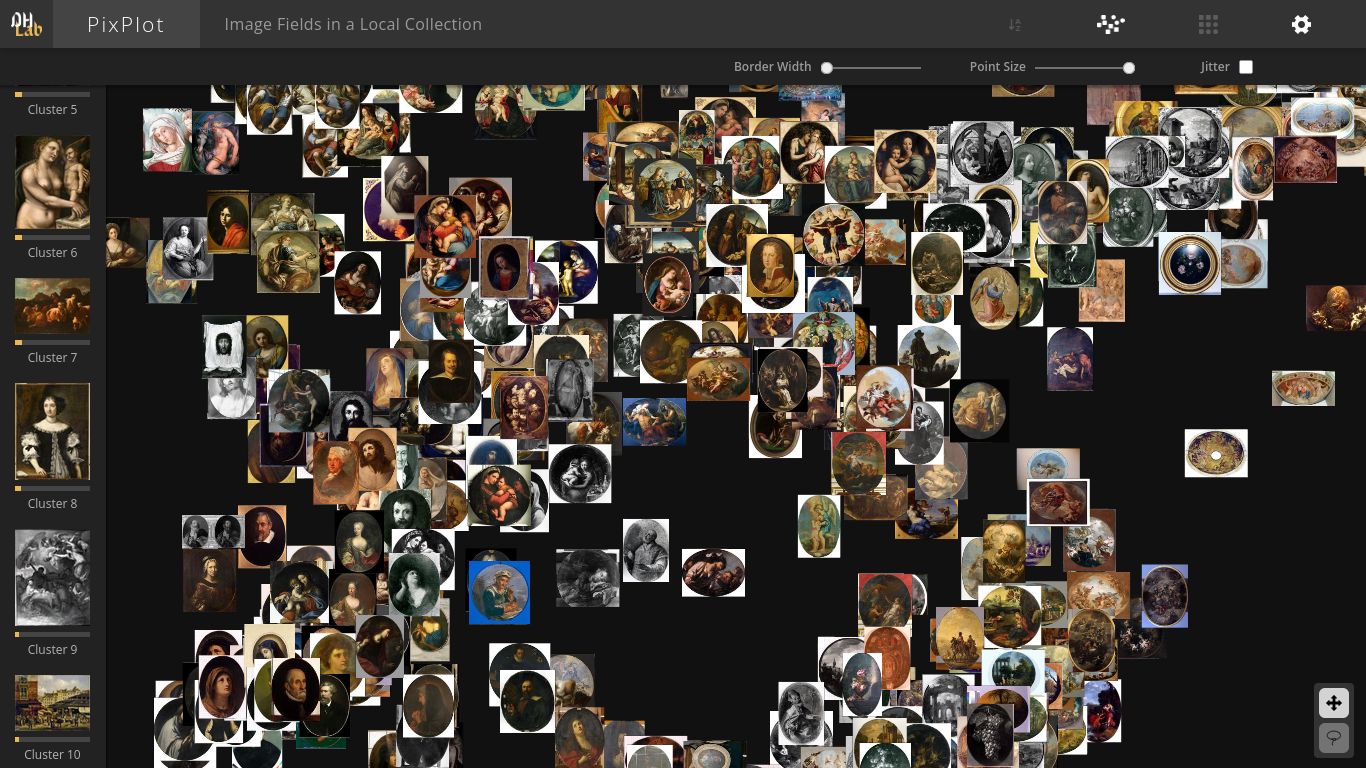
\includegraphics[width=1\textwidth]{annexes/figures/PP-ronds.png}
    \caption{Cluster des tableaux aux formats inhabituels (circulaire, ovale, hexagonal) dans l'angle inférieur droit de la visualisation du RETIF dans PixPlot.}
    \label{fig:PP-ronds}
\end{figure}

\section{Visualisation du corpus dans Panoptic}

\begin{figure}[H]
    \centering
    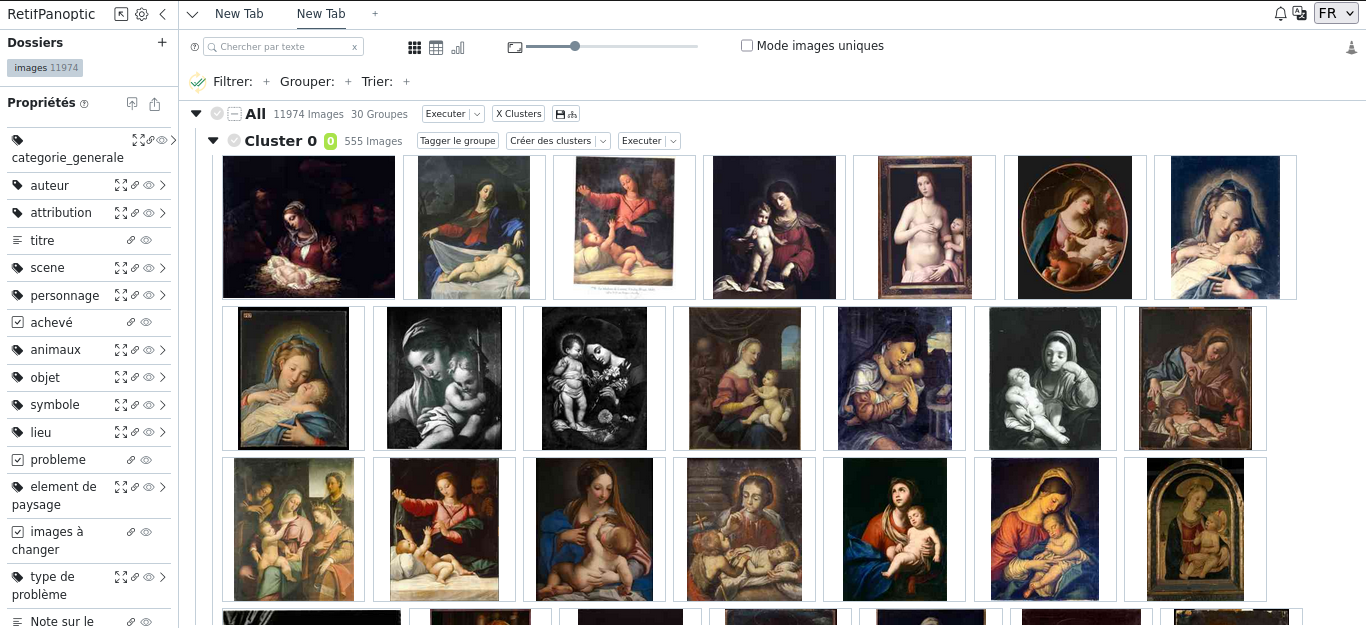
\includegraphics[width=1\textwidth]{annexes/figures/Pa-Vierges.png}
    \caption{Cluster des Vierge à l'Enfant dans Panoptic.}
    \label{fig:Pa-Vierges}
\end{figure}

\begin{figure}[H]
    \centering
    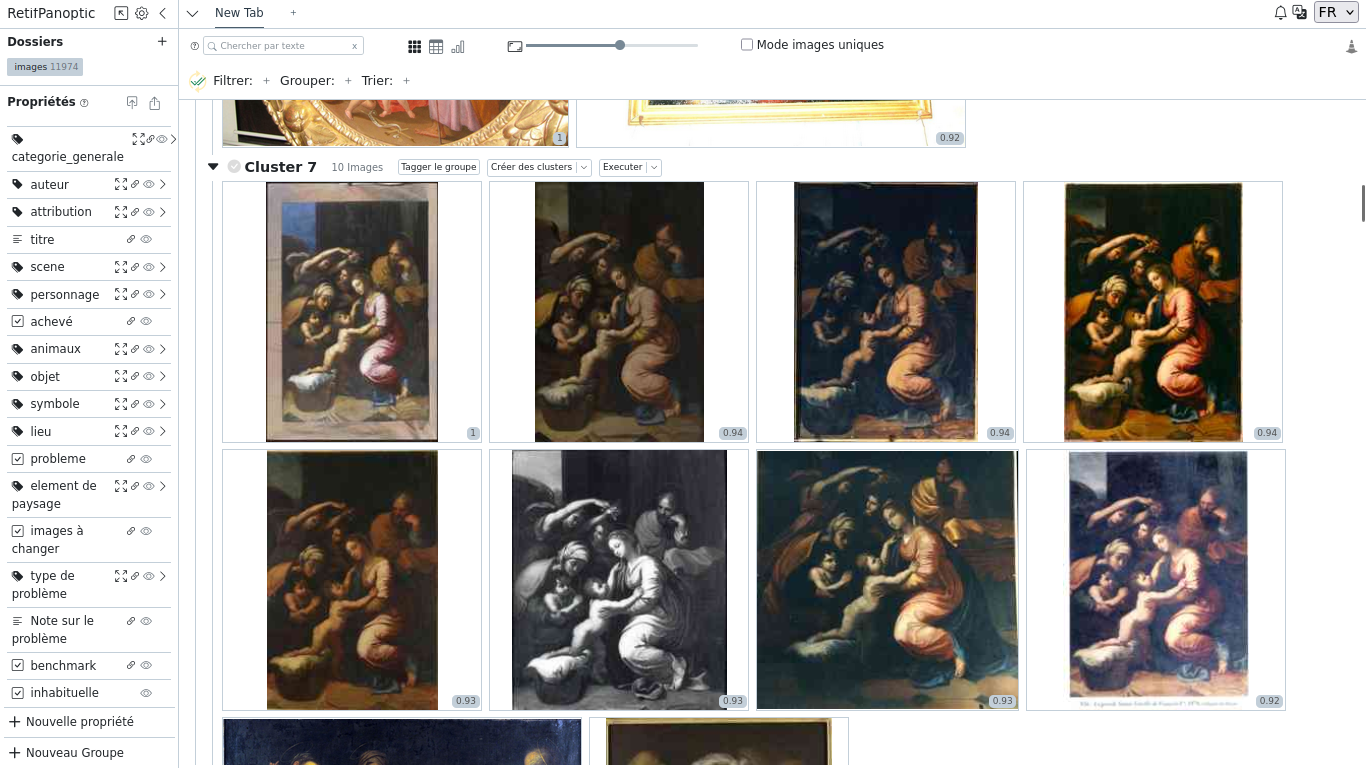
\includegraphics[width=1\textwidth]{annexes/figures/Pa-F1er.png}
    \caption{Les copies de la Sainte Famille de François 1er de Raphaël rassemblées dans Panoptic}
    \label{fig:Pa-F1er}
\end{figure}

\begin{figure}[H]
    \centering
    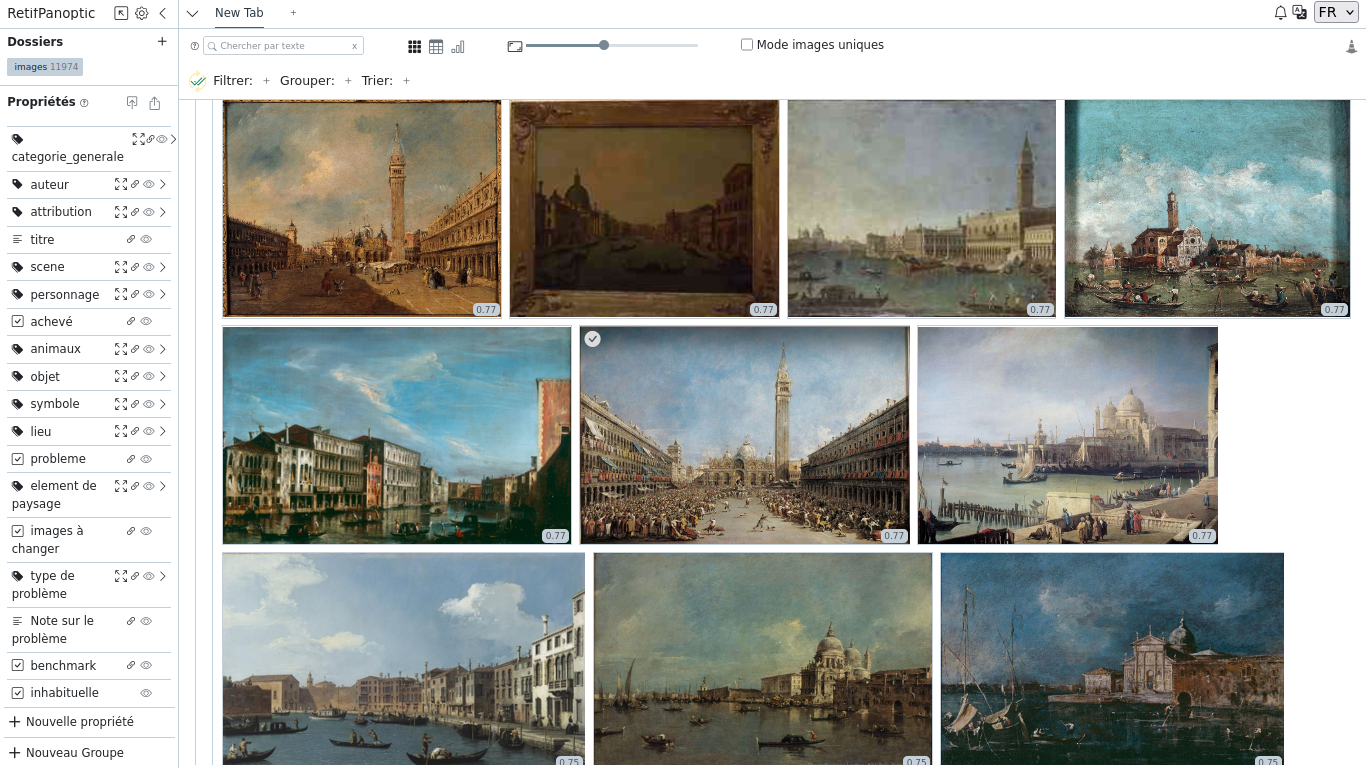
\includegraphics[width=1\textwidth]{annexes/figures/Pa-Venice.png}
    \caption{Une recherche CLIP avec le terme "Venice" dans Panoptic}
    \label{fig:Pa-Venice}
\end{figure}

\section[Statistiques d'indexation]{Statistiques après l'expérimentation d'indexation avec Panoptic}

Ces graphiques sont disponibles au lien suivant : \url{https://public.tableau.com/app/profile/pierre.husson/viz/AGORHA-RETIF/UtilisationdeGarnierdansAgorha}

\begin{figure}[H]
    \centering
    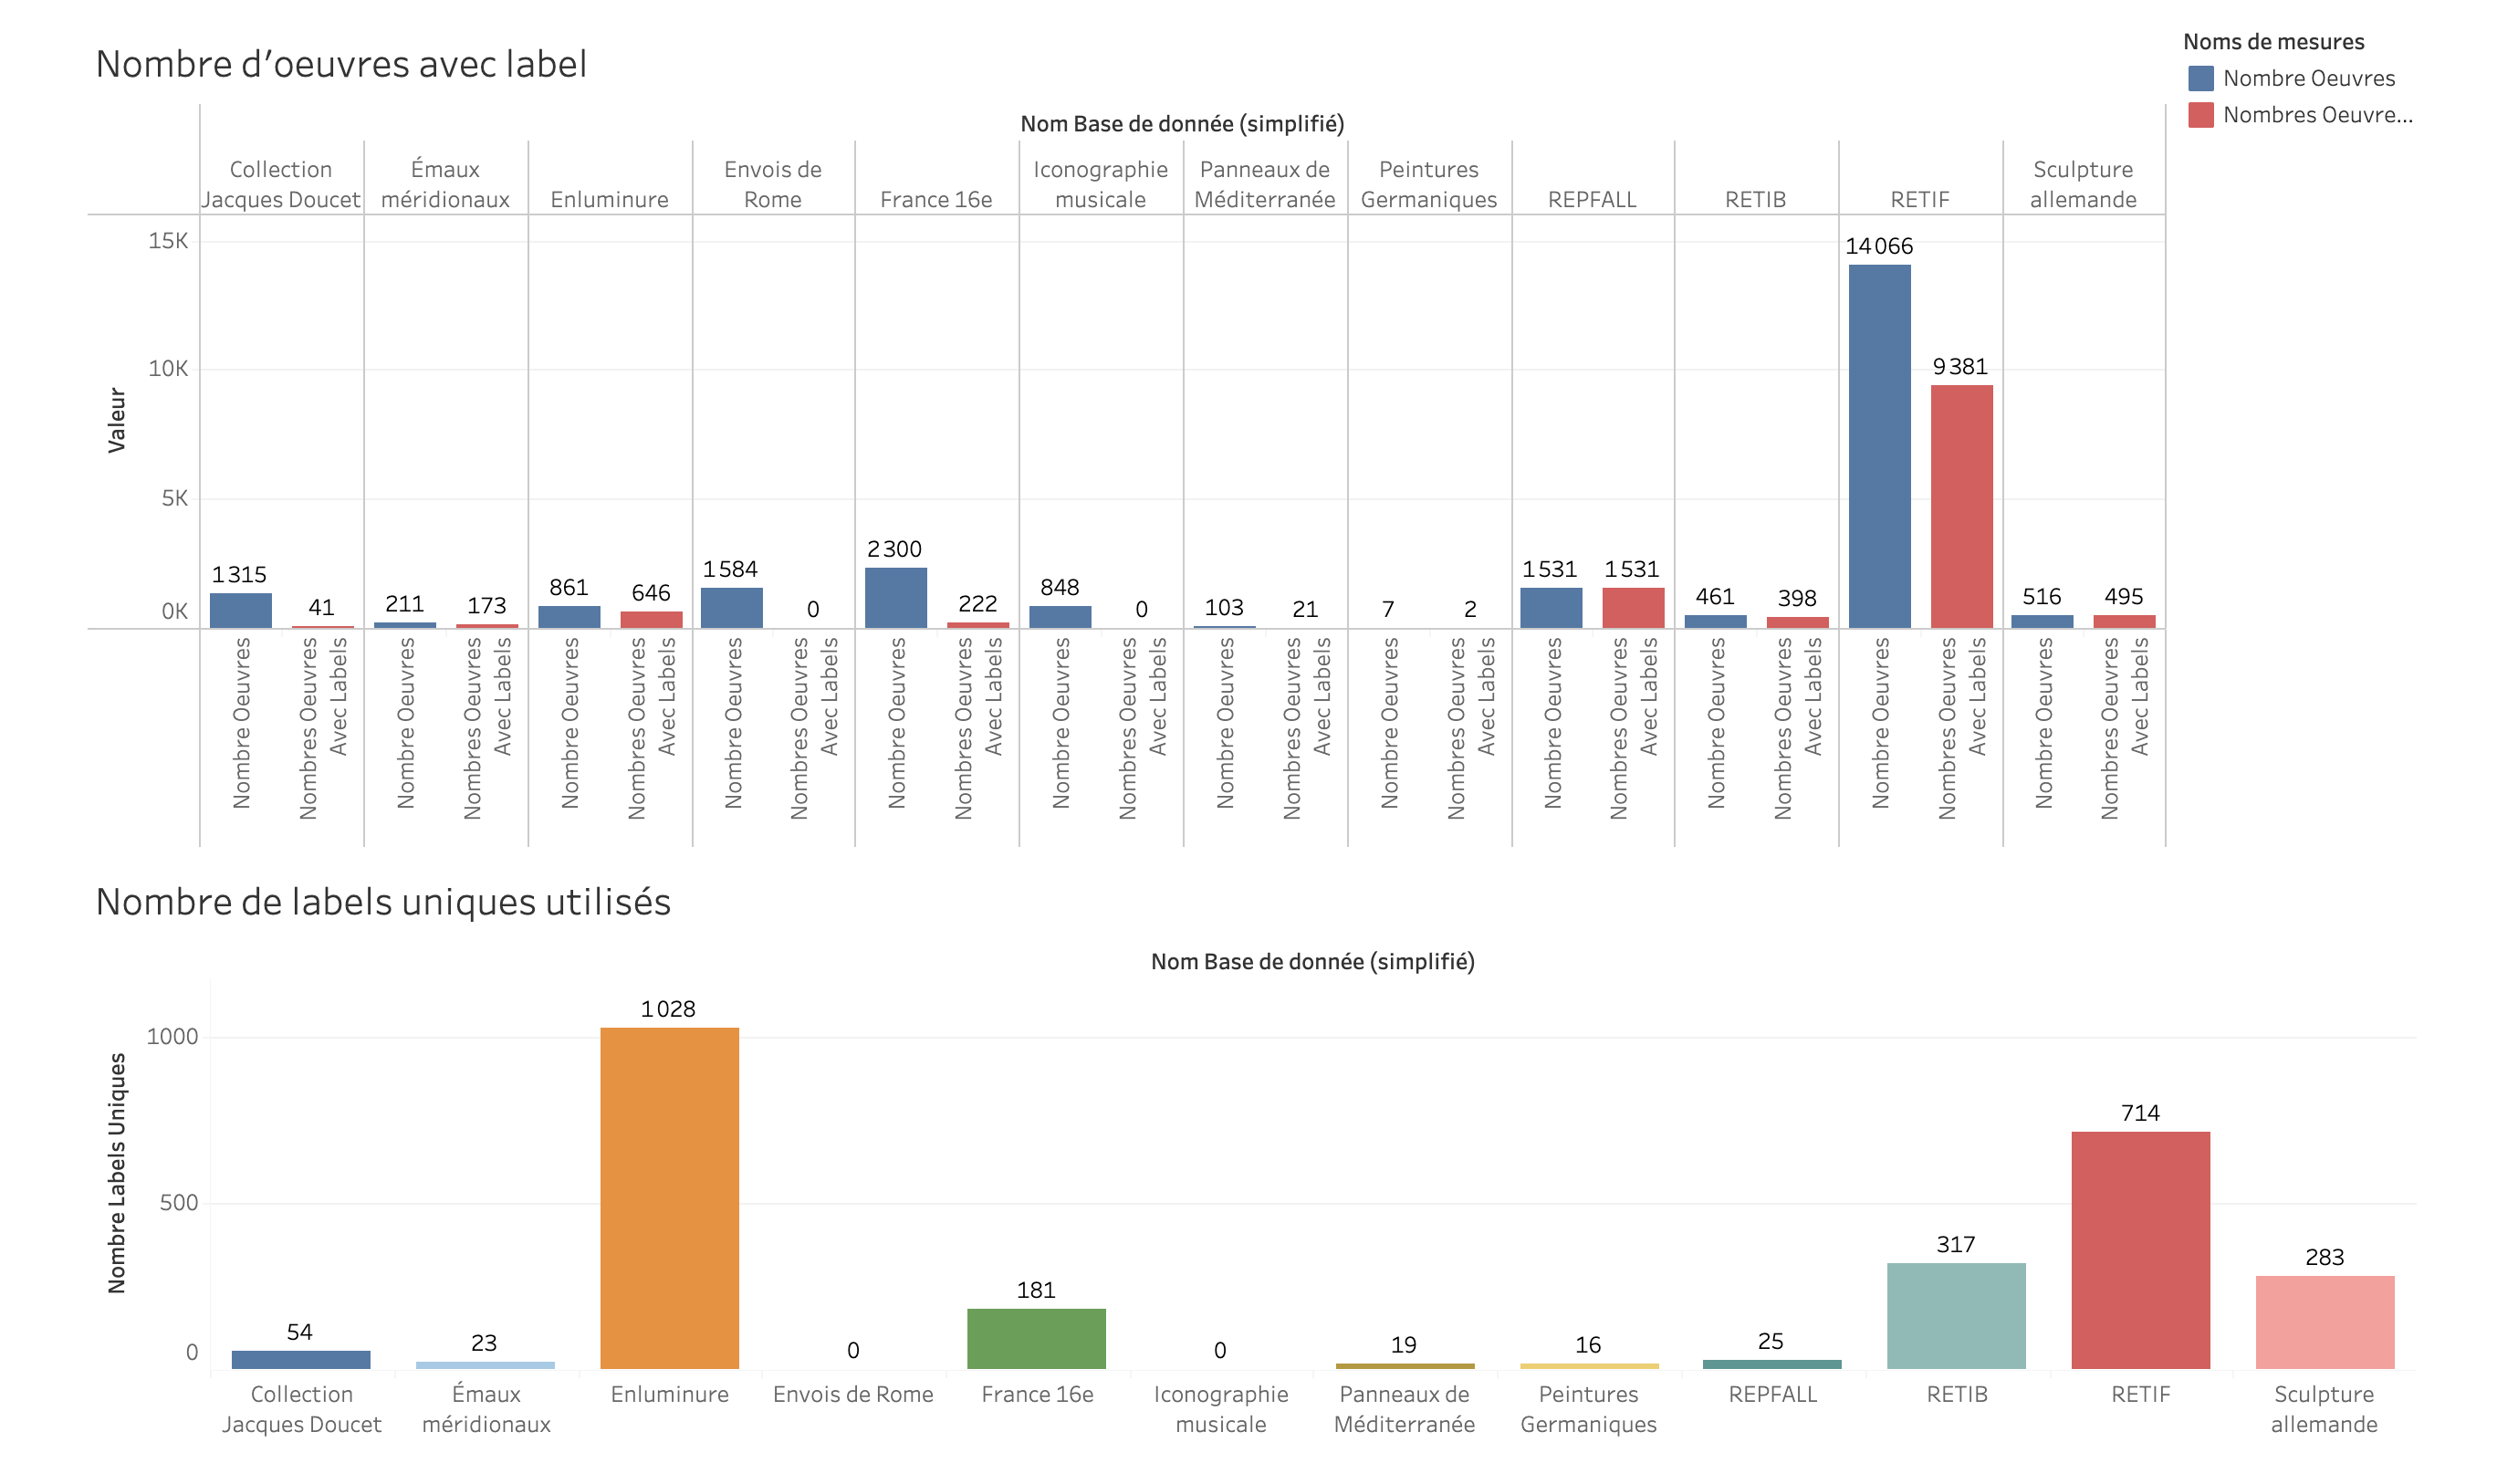
\includegraphics[height=0.4\textheight]{annexes/stats/graphiqueGarnier2A.png}
    \caption{Graphiques montrant le nombre de notices indexées avec au moins un label dans 12 bases d'AGORHA, et le nombre de labels distincts utilisés par bases.}
    \label{stat:Garnier2A}
\end{figure}

\begin{figure}[H]
    \centering
    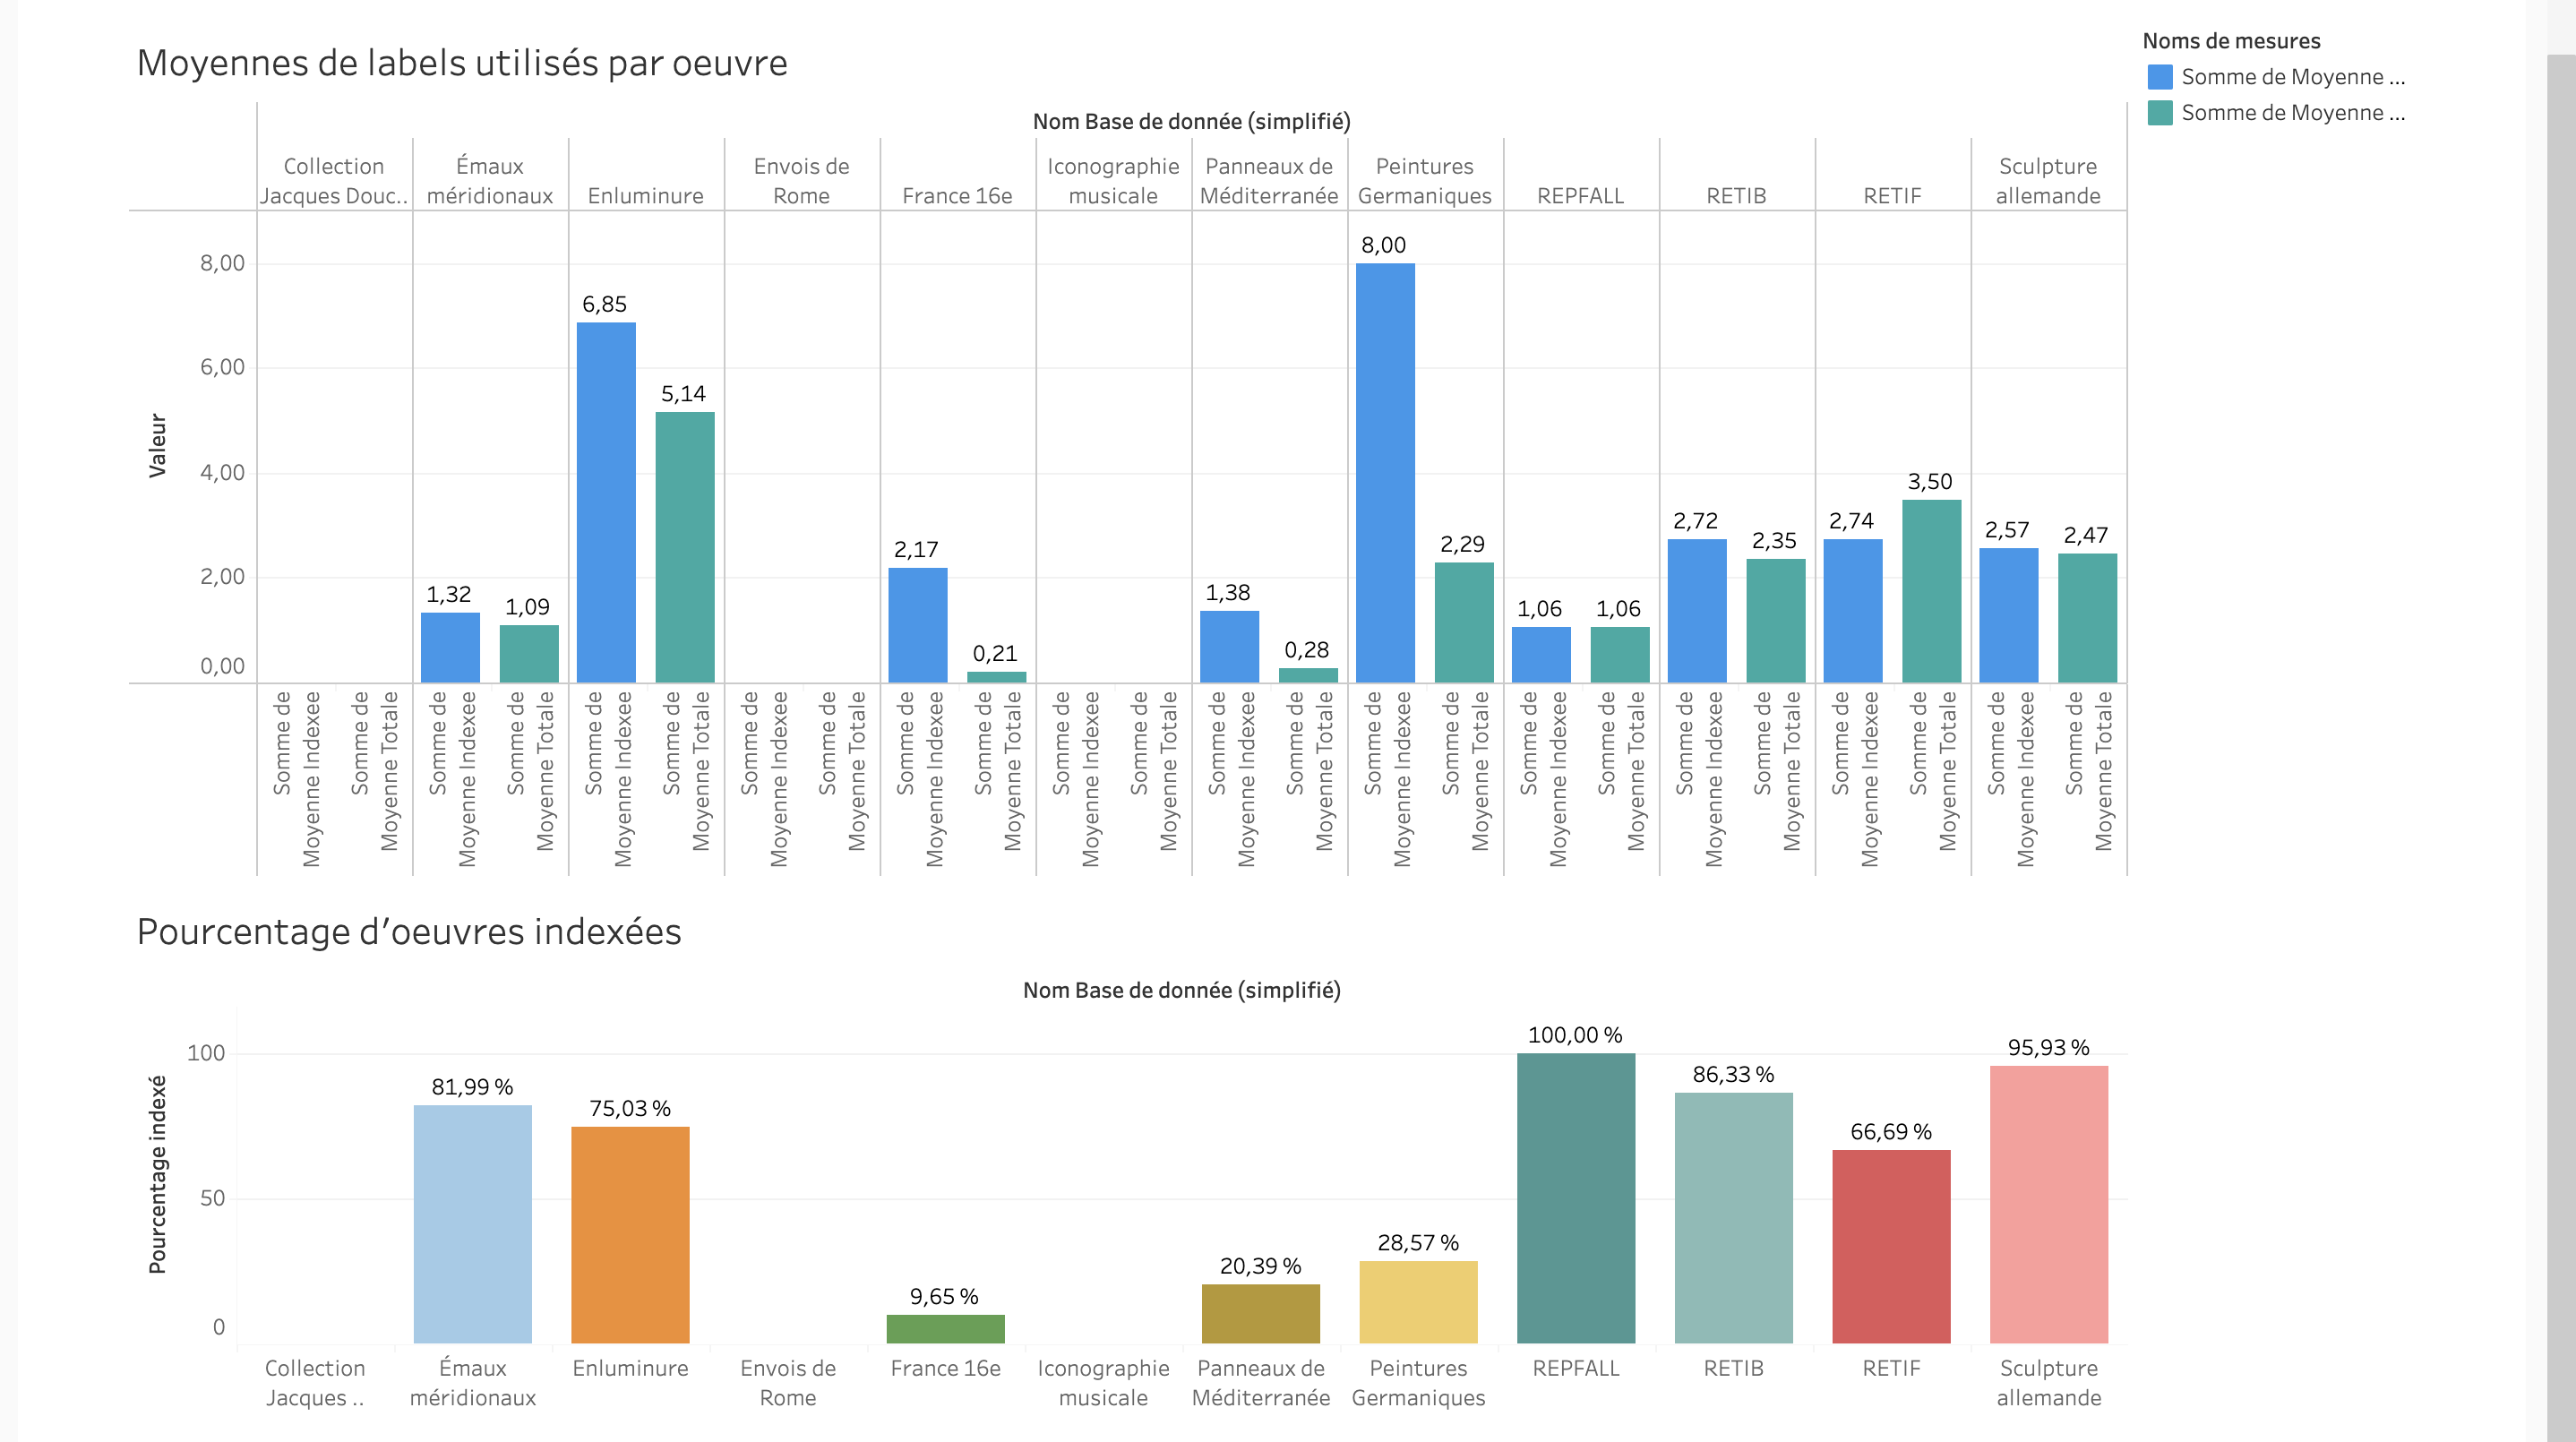
\includegraphics[height=0.4\textheight]{annexes/stats/graphiqueGarnier2B.png}
    \caption{Graphique montrant la moyenne de labels utilisés par notices dans 12 bases d'AGORHA, pour les oeuvres indexées et toutes les oeuvres ; et le pourcentage de d'oeuvres qui possèdent au moins un label par base de données.}
    \label{stat:Garnier2B}
\end{figure}